%%----------------------------------------------------------------------------
%% Onderzoekstechnieken: Het onderzoeksproces
%%----------------------------------------------------------------------------

\documentclass[aspectratio=169]{beamer}

%==============================================================================
% Aanloop
%==============================================================================

%---------- Vormgeving --------------------------------------------------------

\usetheme{hogent}

\usecolortheme{hgwhite} % witte achtergrond, zwarte tekst

\usepackage{graphicx,multicol}
\usepackage{comment,enumerate,hyperref}
\usepackage{amsmath,amsfonts,amssymb}
\usepackage[dutch]{babel}
\usepackage{multirow}
\usepackage{eurosym}
\usepackage{listings}
\usepackage{textcomp}
\usepackage{framed}
\usepackage{wrapfig}
\usepackage{tabu} %needed for \tabulinesep

%---------- Configuratie ------------------------------------------------------

\usetikzlibrary{arrows,shapes,backgrounds,positioning,shadows}

%---------- Commando-definities -----------------------------------------------

\newcommand{\tabitem}{~~\llap{\textbullet}~~}
\newcommand{\alertbox}[2][hgblue]{%
  \setbeamercolor{alertbox}{bg=#1,fg=white}
  \begin{beamercolorbox}[sep=2pt,center]{alertbox}
    \textbf{#2}
  \end{beamercolorbox}
}

%---------- Info over de presentatie ------------------------------------------

\title{Hst 2. Het onderzoeksproces}
\subtitle{Onderzoekstechnieken}
\author{Jens Buysse \and Wim {De Bruyn} \and Pieter-Jan Maenhout \and Bert {Van Vreckem}}
\date{AJ 2019-2020}

%==============================================================================
% Inhoud presentatie
%==============================================================================

\begin{document}

\begin{frame}
  \maketitle
\end{frame}

\begin{frame}
  \frametitle{What's on the menu today?}
  
  \tableofcontents
\end{frame}

\begin{frame}
  \frametitle{Leerdoelen}
  
  \begin{itemize}
    \item De wetenschappelijke methode
    \item Onderzoeksproces
    \item Variabelen en meetniveaus
    \item Steekproeven
    \item Basisbegrippen
  \end{itemize}
\end{frame}

\section{De wetenschappelijke methode}


\begin{frame}[plain]
  \bfseries\Large
  No matter how many instances of white swans we may have observed, this does not justify the conclusion that all swans are white
  
  \bigskip
  
  ---Karl Popper
\end{frame}

\begin{frame}[plain]
  \centering
  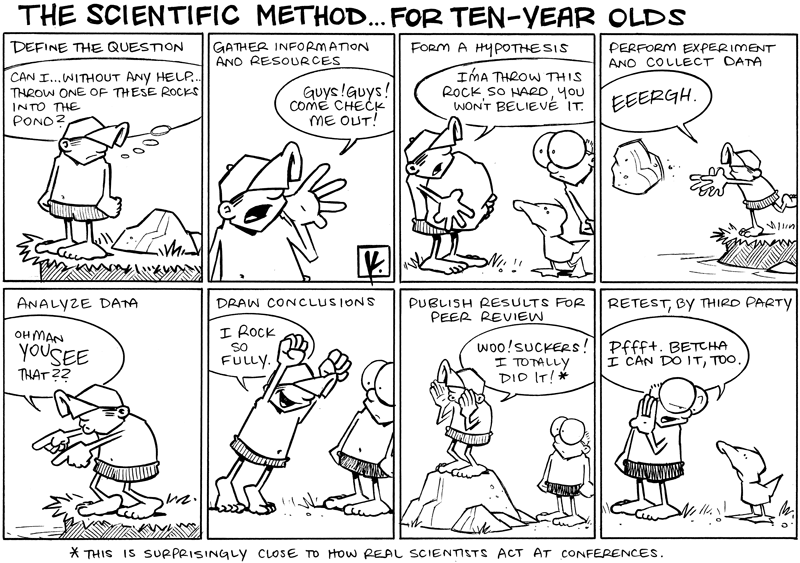
\includegraphics[height=\textheight]{les1-01}
\end{frame}

\begin{frame}
  \frametitle{Hoe vergaren we kennis?}
  
  \centering
  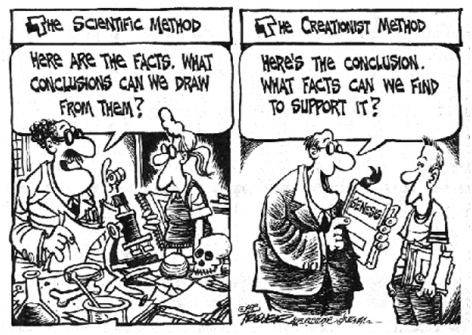
\includegraphics[height=.8\textheight]{les1-02}
\end{frame}

\begin{frame}[plain,c]
  \begin{columns}
    \column{\dimexpr\paperwidth}
    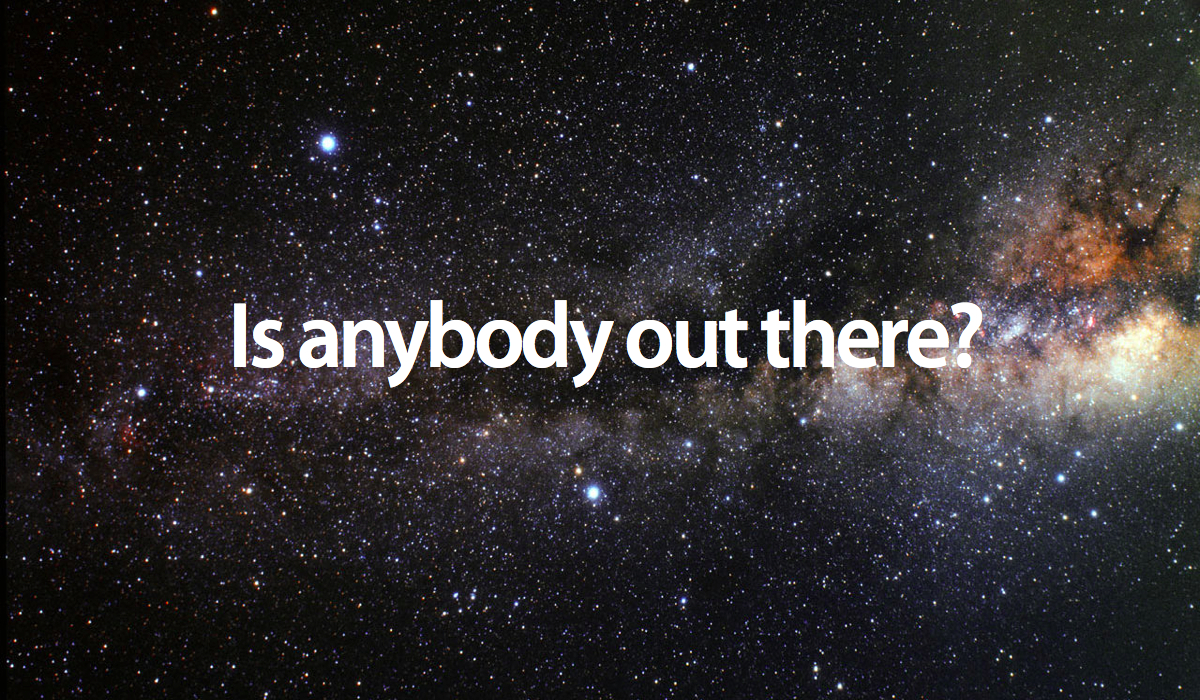
\includegraphics[width=\paperwidth]{les1-03}
  \end{columns}
\end{frame}

\begin{frame}
  \frametitle{Hoe vergaren we kennis?}
  
  \begin{columns}[c]
    
    \column{.5\textwidth}
    Niet-wetenschappelijke methode
    \begin{itemize}
      \item ``Mijn buikgevoel zegt van wel''
      \item ``Mijn vader zegt van wel, dus moet het wel''
      \item ``Er zijn verschillende beelden van UFO's en dus kan het niet anders''
      \item ``Ik heb het gelezen op het Internet!''
    \end{itemize}
    
    \pause
    
    \column{.5\textwidth}
    Wetenschappelijke methode
    \begin{itemize}
      \item ``Er zijn veel planeten''
      \item ``Moleculen nodig voor leven vind je overal''
      \item $\Rightarrow$ ``Dus ik zou verwonderd zijn indien er geen leven is''
      \item \textbf{Maar er is nog geen bewijs voor}
    \end{itemize}
    
  \end{columns}
\end{frame}

\begin{frame}
  \frametitle{Kunnen varkens vliegen?}
  % Bedoeling is hier de klas in 3 te delen: ene groep moet aantonen dat varkens kunnen vliegen op autoritaire wijze (bv. Bij boer Mcdonald gaan en navraag), de tweede op deductieve wijze (varkens zijn deel van gewervelden, sommige gewervelden hebben vleugels en dus .. (maar dus met verkeerde conclusie) en de derde tracht dit op wetenschappelijke methode. Hier kan voor deductie ook ik kan in pyama, pyama kan in koffer, dus ik kan in koffer gebruikt worden.
  \centering
  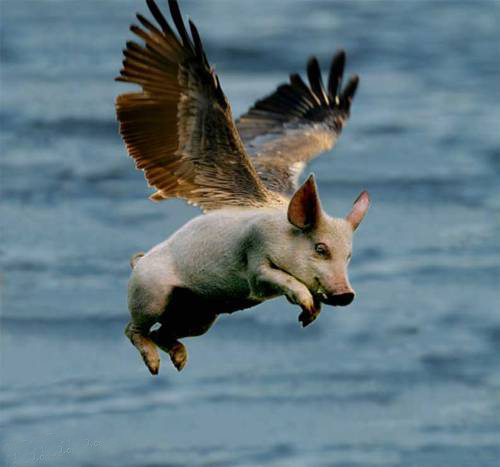
\includegraphics[height=.8\textheight]{les1-04}
\end{frame}

\begin{frame}
  \frametitle{De wetenschappelijke methode}
  
  Aan de hand van \textbf{empirisch onderzoek} zijn we geïnteresseerd in volgende zaken:
  
  \begin{enumerate}
    \item Exploratie
    \item Beschrijving
    \item Voorspelling
    \item Controle
  \end{enumerate}
\end{frame}

\begin{frame}
  \frametitle{De wetenschappelijke methode}
  
  \begin{columns}[c]
    
    \column{0.8\textwidth}
    \begin{itemize}
      \item Generalisatie
      \begin{itemize}
        \item Bv. ``Agressie komt vaak voor in deze bevolkingsgroep''
      \end{itemize}
      \item Verstaan, begrijpen
      \begin{itemize}
        \item Er is een verband tussen frustratie en agressie
        \item Theorieontwikkeling
      \end{itemize}
    \end{itemize}
    
    \column{0.2\textwidth}
    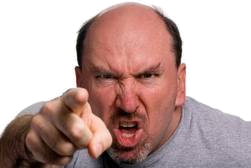
\includegraphics[width=\textwidth]{les1-05}
    \vspace*{1cm}
    
\includegraphics[width=\textwidth]{les1-06}
    
  \end{columns}
\end{frame}

\section{Het onderzoeksproces}


\begin{frame}
  \frametitle{Het onderzoeksproces}
  
  \begin{columns}
    \column{\dimexpr\paperwidth}
    
    \begin{center}
      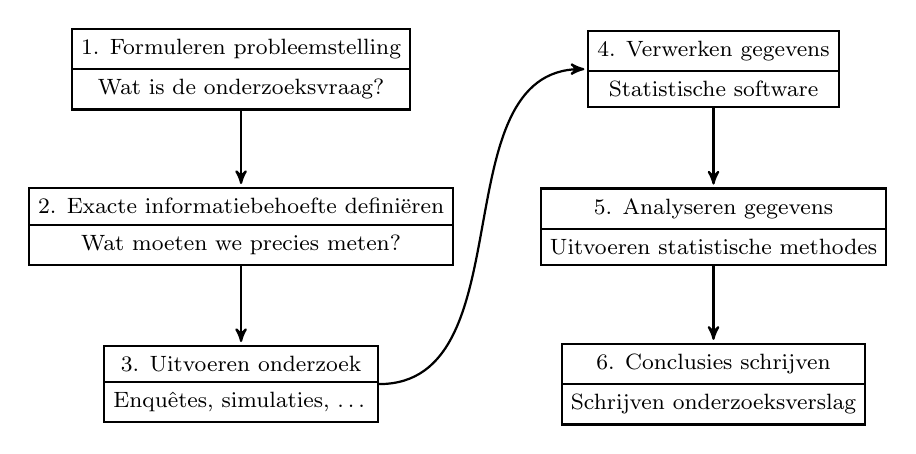
\begin{tikzpicture}[
      auto,
      thick,
      ->,
      >=stealth',
      shorten >=1pt,
      node distance=2cm,
      fase/.style={
        shape=rectangle split,
        rectangle split parts=2,
        ,
        draw}]
      
      
      \node[fase] (1) {
        \footnotesize{1. Formuleren probleemstelling}
        \nodepart{second}
        \footnotesize{Wat is de onderzoeksvraag?}
      };
      \uncover<2->{\node[fase] (2) [below of=1] {
          \footnotesize{2. Exacte informatiebehoefte definiëren}
          \nodepart{second}
          \footnotesize{Wat moeten we precies meten?}
        };}
      \uncover<3->{\node[fase] (3) [below of=2] {
          \footnotesize{3. Uitvoeren onderzoek}
          \nodepart{second}
          \footnotesize{Enquêtes, simulaties, \ldots}
        };}
      \uncover<4->{\node[fase] (4) [right of=1, node distance=6cm] {
          \footnotesize{4. Verwerken gegevens}
          \nodepart{second}
          \footnotesize{Statistische software}
        };}
      \uncover<5->{\node[fase] (5) [below of=4] {
          \footnotesize{5. Analyseren gegevens}
          \nodepart{second}
          \footnotesize{Uitvoeren statistische methodes}
        };}
      \uncover<6->{\node[fase] (6) [below of=5] {
          \footnotesize{6. Conclusies schrijven}
          \nodepart{second}
          \footnotesize{Schrijven onderzoeksverslag}
        };}
      
      \uncover<2->{\draw (1) -- (2);}
      \uncover<3->{\draw (2) -- (3);}
      \uncover<4->{\draw (3.east) to [out=0,in=180] (4.west);}
      \uncover<5->{\draw (4) -- (5);}
      \uncover<6->{\draw (5) -- (6);}
      \end{tikzpicture}
    \end{center}
  \end{columns}
  
\end{frame}

\section{Basisconcepten in onderzoek}

\begin{frame}
  \frametitle{Variabelen en waarden}
  
  \begin{description}
    \item[Variabele] Algemene eigenschap van een object waardoor we objecten van elkaar kunnen onderscheiden
    \item[Waarde] Specifieke eigenschap, invulling voor die variabele
  \end{description}
  
  \vspace{1cm}
  
  \begin{columns}[c]
    \column{.6\textwidth}
    \centering
    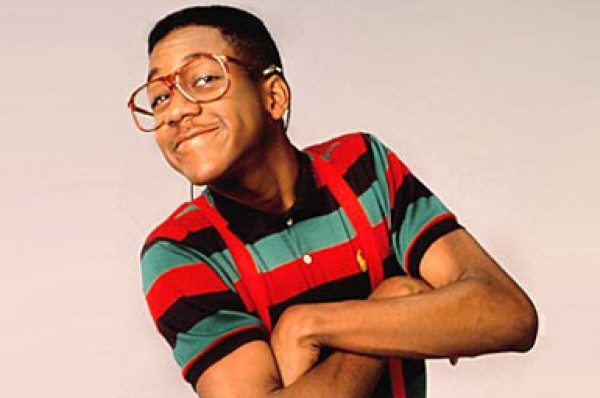
\includegraphics[width=.7\textwidth]{les1-07}
    
    \column{.4\textwidth}
    \fbox{\parbox{3cm}{%
        \scriptsize
        Variabele: geslacht\\
        Waarde: man
    }}\\
    \vspace{.5cm}
    \fbox{\parbox{3cm}{%
        \scriptsize
        Variabele: hoogte\\
        Waarde: 180cm
    }}\\
    \vspace{.5cm}
    \fbox{\parbox{3cm}{%
        \scriptsize
        Variabele: grappig\\
        Waarde: nee
    }}
    
  \end{columns}
\end{frame}

\begin{frame}
  \frametitle{Meetniveaus}
  
  \begin{itemize}
    \item = Types van variabelen
    \item Bepalen meest geschikte methode voor analyseren
    \begin{itemize}
      \item visualisatiemethoden
      \item centrum- en spreidingsmaten
      \item verband tussen variabelen onderzoeken
    \end{itemize}
  \end{itemize}
  
\end{frame}

\begin{frame}
  \frametitle{Meetniveaus}
  \framesubtitle{Kwalitatief vs kwantitatief}
  
  \begin{center}
    \begin{tabular}{ll}
    	\textbf{Kwalitatief}       & \textbf{Kwantitatief}    \\
    	\hline
    	Niet noodzakelijk numeriek & Getal + meeteenheid      \\
    	Beperkt aantal waarden     & Vele waarden, vaak uniek
    \end{tabular}
  \end{center}

  \bigskip

  Kwantitatieve variabelen bevatten vaak het resultaat van een \textbf{meting}
\end{frame}

\begin{frame}
  \frametitle{Meetniveaus}
  \framesubtitle{Kwalitatieve schalen}
  
  \begin{description}
    \item[Nominaal] Categorieën.
    
      Bv. Geslacht, ras, land, vorm, \ldots
      
    \item[Ordinaal] Volgorde, rang.
    
      Bv. militaire rang, opleidingsniveau, \ldots
  \end{description}
  
\end{frame}

\begin{frame}
  \frametitle{Meetniveaus}
  \framesubtitle{Kwantitatieve schalen}
  
  \begin{description}
    \item[Interval] Geen vast nulpunt $\Rightarrow$ geen verhoudingen
    
    bv. °C, °F
    
    \item[Ratio] Absoluut nulpunt $\Rightarrow$ verhoudingen
    
    bv. Afstand (m), energie (J), massa (kg) \ldots\\
  \end{description}

  \bigskip

  Verhoudingen:
  
  \begin{itemize}
    \item 20 m is 1/3 of $\sim$33\% langer dan 15 m
    \item 20 °C is \textbf{NIET} 1/3 warmer dan 15 °C (zet eens om in °F)

  \end{itemize}    
  
\end{frame}

\begin{frame}
  \frametitle{Verbanden tussen variabelen}
  
  Er is een verband tussen variabelen als hun waarden \textbf{systematisch} veranderen.
  
  \begin{center}
    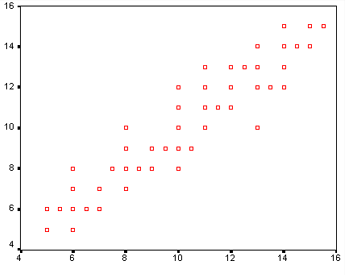
\includegraphics[height=4cm]{les1-08a}
    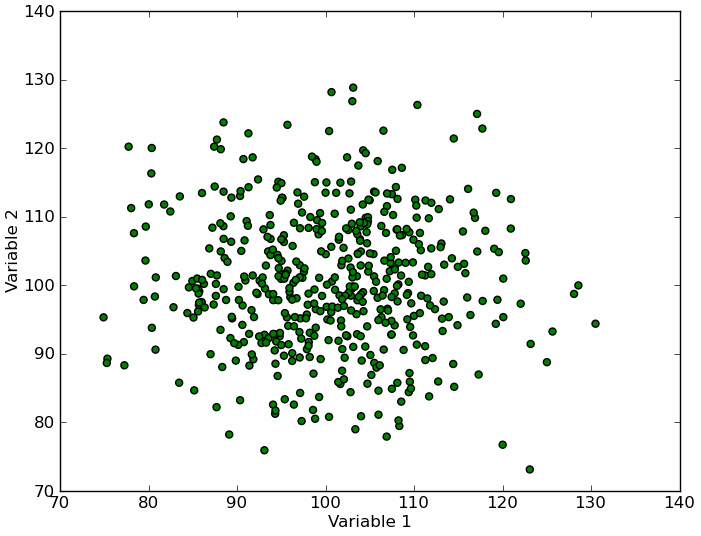
\includegraphics[height=4cm]{les1-08b}
  \end{center}
\end{frame}

\begin{frame}
  \frametitle{Verbanden tussen variabelen: voorbeeld}
  
  Is er een verband tussen soort cola en waardering van de smaak?
  
  \begin{columns}
    \column{0.99\textwidth}
    \begin{table}
      \centering
      \begin{tabular}{l||c|c||c}
        & Pepsi & Coca Cola & Totaal \\
        \hline \hline
        Lekker & 56 & 24 & \alert<2>{80} \\
        \hline
        Niet lekker & 14 & 6 & \alert<2>{20} \\
        \hline \hline
        Totaal & \alert<2>{70} & \alert<2>{30} & \alert<2>{100}
      \end{tabular}
    \end{table}
    
    \only<2>{Marginale totalen}
    
    \column{.01\textwidth}
    \hspace*{-2cm}
    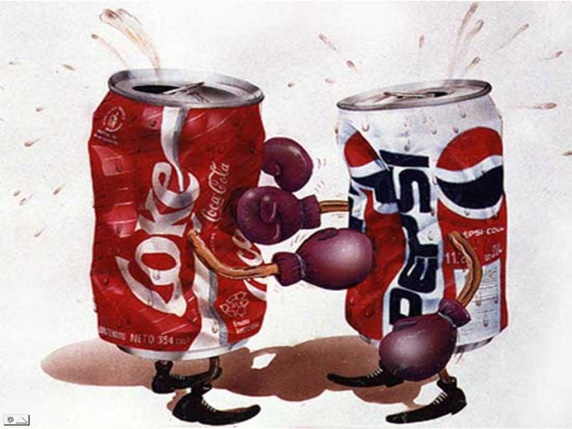
\includegraphics[width=2cm]{les1-09}
  \end{columns}
\end{frame}

\begin{frame}
  \frametitle{Oorzakelijke verbanden}
  
  We zijn vooral op zoek naar \textbf{oorzakelijke verbanden}, bv.
  
  \begin{itemize}
    \item Frustratie leidt tot agressie
    \item Alcohol leidt tot minder oplettendheid
    \item \ldots
  \end{itemize}
  
  \begin{description}
    \item[Oorzaak] Onafhankelijke variabele
    \item[Gevolg] Afhankelijke variabele
  \end{description}
\end{frame}

\begin{frame}
  \frametitle{Oorzakelijke verbanden}
  \framesubtitle{Valse correlatie of ``Spurious correlation''}
  
  \alertbox{\textcolor{yellow}{Let op!} Een verband tussen variabelen duidt niet noodzakelijk op een oorzakelijk verband!}
  
  \bigskip
  
  \begin{columns}
    \begin{column}{.8\textwidth}
      Verband tussen:
      
      \begin{itemize}
        \item Gaming en geweld
        \item Vaccinaties en autisme
        \item Drinken van cola light en obesitas
        \item \ldots
      \end{itemize}
      
    \end{column}
    \begin{column}{.2\textwidth}
      
\includegraphics[height=2.5cm]{les1-10}
    \end{column}
  \end{columns}

\end{frame}

\begin{frame}[plain]
  \centering
  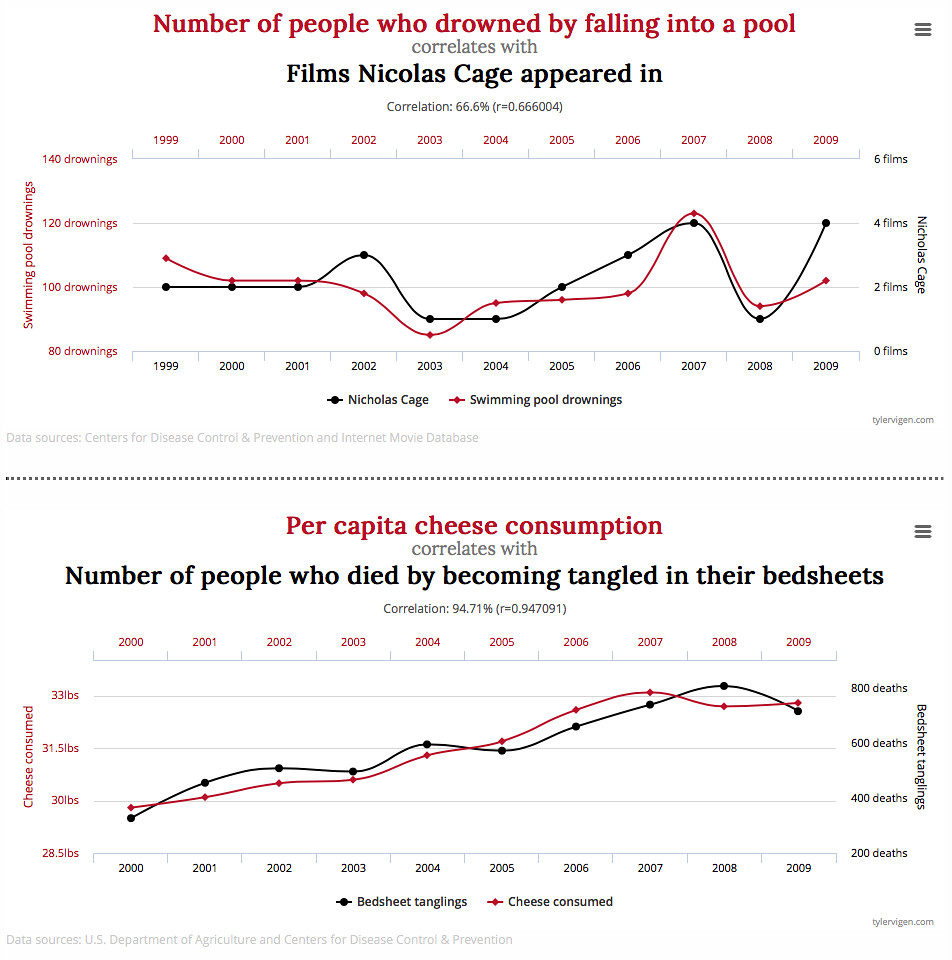
\includegraphics[height=\textheight]{hst1-spurious-correlation}
\end{frame}

\section{Steekproefonderzoek}


\begin{frame}
  \large\bfseries
  
  USA Today has come out with a new survey. Apparently, three out of every four people make up 75\% of the population
  
  \bigskip
  
  ---David Letterman
  
\end{frame}

\begin{frame}
  \frametitle{Stel, je wil een vriendengroep analyseren}
  
  Vragen die je kan stellen:
  
  \begin{itemize}
    \item Hoe groot mijn vrienden?
    \item Hoeveel wegen ze?
    \item Hoe veilig maken ze hun woonomgeving?
    \item Hebben ze familie?
    \item \ldots
  \end{itemize}

\end{frame}

\begin{frame}[plain]
  \frametitle{Populatie}
  
  \begin{figure}
    \centering
    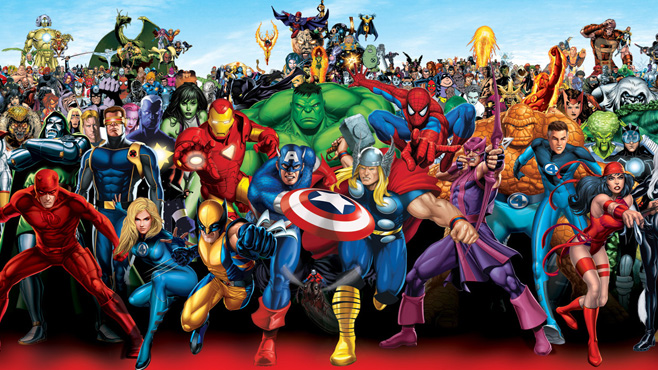
\includegraphics[height=.9\textheight]{les5-heroes.jpg}
    \label{fig:les5-heroes}
  \end{figure}
  
\end{frame}


\begin{frame}[plain]
  \frametitle{Steekproef en Populatie}
  
  \begin{description}
    \item[Populatie] de verzameling van alle objecten/personen/$\ldots$ die men wil onderzoeken
    \item[Steekproef] een \textit{deelverzameling} van de populatie waar men metingen op zal uitvoeren
  \end{description}
  
  \begin{center}
    \begin{tikzpicture}[scale=.55]
    \fill[hgyellow] (2,2) ellipse (4cm and 2cm) ;
    \fill[hgorange] (1.5,2) ellipse (2cm and 1cm) ;
    \node[draw=none,minimum size=1cm,inner sep=0pt] at (3,0.5) {populatie};
    \node[draw=none,minimum size=1cm,inner sep=0pt] at (2.5,2) {steekproef};
    \end{tikzpicture}
  \end{center}

  \alertbox{Onder bepaalde omstandigheden zijn de resultaten voor een steekproef representatief voor de populatie.}
\end{frame}

\begin{frame}
  \frametitle{Steekproef en Populatie}
  
  Een steekproef is makkelijker te analyseren dan de hele populatie
  
  \centering
  \begin{tikzpicture}[xscale=4,yscale=2]
  \draw (0,2) -- (0,0);
  \foreach \num/\label in {0/0, 0.2/20, .4/40, .6/60, .8/80, 1/100, 1.2/120, 1.4/140, 1.6/160, 1.8/180, 2/200}{%
    \draw (0, \num) -- (2.5, \num);
    \draw[shift={(0, \num)}] (1pt,0pt) -- (-1pt,0pt) node[left] {\scriptsize \label};
  }
  
  \node[anchor=north] (hero1) at (0.3,1.5)
  {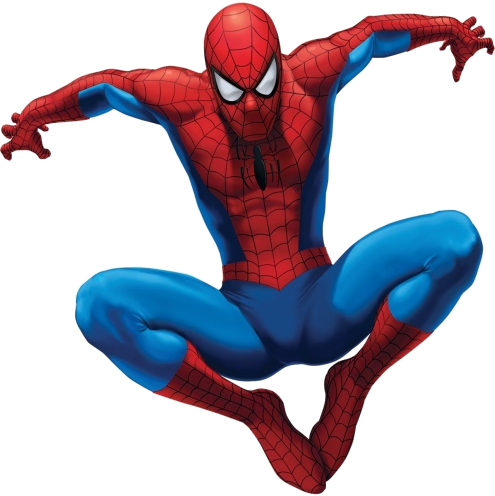
\includegraphics[height=2.9cm]{les2-hero-1}};
  \node[anchor=north] (hero2) at (0.8,2.05)
  {
\includegraphics[height=4cm]{les2-hero-2}};
  \node[anchor=north] (hero3) at (1.3,1.575)
  {
\includegraphics[height=3.1cm]{les2-hero-3}};
  \node[anchor=north] (hero4) at (1.8,2.1)
  {
\includegraphics[height=4.1cm]{les2-hero-4}};
  \node[anchor=north] (hero5) at (2.3,1.95)
  {
\includegraphics[height=3.8cm]{les2-hero-5}};
  
  \node (size1) at (0.3, 1.5) {\scriptsize 141 cm};
  \node (size2) at (0.8, 2.1) {\scriptsize 198 cm};
  \node (size3) at (1.3, 1.51) {\scriptsize 143 cm};
  \node (size4) at (1.8, 2.15) {\scriptsize 201 cm};
  \node (size5) at (2.3, 1.95) {\scriptsize 184 cm};
  \end{tikzpicture}
\end{frame}


\begin{frame}
  \frametitle{Methode om tot een steekproef te komen}
  \begin{center}
    \begin{tikzpicture}[
    auto, thick, ->, >=stealth', shorten >=1pt, node distance=1.5cm,
    fase/.style={ shape=rectangle, fill=hgblue, text=white, draw}
    ]
    
    \node[fase] (1) { Definitie van populatie };
    \node[fase] (2) [below of=1] { Bepalen van steekproefkader };
    \node[fase] (3) [below of=2] { Keuze steekproefmethode (budget en tijd) };
    
    \draw (1) -- (2);
    \draw (2) -- (3);
    \end{tikzpicture}
  \end{center}
  
\end{frame}

\begin{frame}
  \frametitle{Gestratificeerd naar variabelen}
  
  \begin{center}
    \begin{tabular}{l|cccc|c}
      & \multicolumn{4}{c|}{\textbf{Leeftijd}} & \\
      Geslacht & $\le 18$ & $]18,25]$ & $]25, 40]$ & $> 40$ & Totaal\\
      \hline
      Vrouw & 500 & 1500 & 1000 & 250 & 3250 \\
      Man   & 400 & 1200 & 800 & 160 & 2560\\
      \hline
      Totaal & 900 & 2700 & 1800 & 410 & 5810
    \end{tabular}
    
    \vspace{.5cm}
    
    \pause
    \begin{tabular}{l|cccc|c}
      & \multicolumn{4}{c|}{\textbf{Leeftijd}} & \\
      Geslacht & $\le 18$ & $]18,25]$ & $]25, 40]$ & $> 40$ & Totaal\\
      \hline
      Vrouw & 50 & 150 & 100 & 25 & 325 \\
      Man   & 40 & 120 & 80 & 16 & 256\\
      \hline
      Totaal & 90 & 270 & 180 & 41 & 581
    \end{tabular}
    
  \end{center}
\end{frame}

\begin{frame}
  \frametitle{Hoe elementen voor een steekproef kiezen?}
  
  \begin{description}
    \item[Aselecte (of random) steekproef]: elk element uit de onderzoekspopulatie heeft een even grote kans om in de steekproef terecht te komen
    \item[Selecte steekproef]: de elementen voor de steekproef worden \textit{niet} random geselecteerd.
    Objecten die \textit{gemakkelijk} kunnen verzameld worden, hebben meer kans om in de steekproef terecht te komen.
    (convenience sampling)
  \end{description}
  
  \begin{center}
    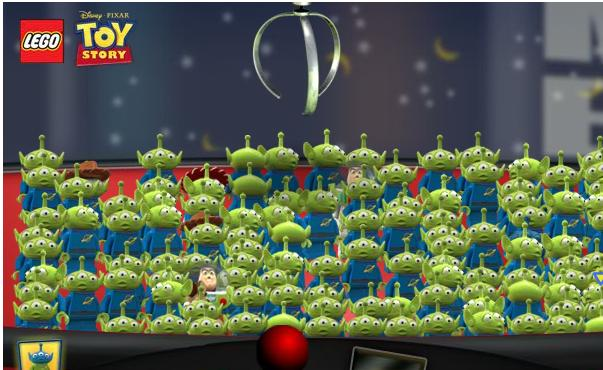
\includegraphics[height=.4\textheight]{les4-aselect}
  \end{center}
\end{frame}

\begin{frame}
  \frametitle{Mogelijke fouten}
  
  Metingen in een steekproef zullen typisch afwijken van de waarde in de hele populatie $\Rightarrow$ Fouten!
  
  \bigskip
  
  \begin{itemize}
    \item Toevallig $\leftrightarrow$ Systematisch
    \item Steekproeffout $\leftrightarrow$ Niet-steekproeffout
  \end{itemize}
\end{frame}

\begin{frame}
  \frametitle{Steekproeffouten}
  
  \begin{itemize}
    \item<+-> Toevallige steekproeffouten
    \begin{itemize}
      \item Puur toeval
    \end{itemize}
    \item<+-> Systematische steekproeffouten
    \begin{itemize}
      \item Online enquête: mensen zonder internet worden uitgesloten
      \item Straatenquête: enkel wie daar op dat moment loopt
      \item Vrijwillige enquête: enkel geïnteresseerden doen mee
    \end{itemize}
  \end{itemize}
\end{frame}

\begin{frame}
  \frametitle{Niet-steekproeffouten}
  \begin{itemize}
    \item<+-> Toevallige niet-steekproeffouten
    \begin{itemize}
      \item Verkeerd aangekruiste antwoorden
    \end{itemize}
    \item<+-> Systematische niet-steekproeffouten
    \begin{itemize}
      \item Slechte of niet geijkte meetapparatuur (slechte weegschaal)
      \item Waarde kan beïnvloed worden door het feit dat je meet
      \item Respondenten liegen (aantal sigaretten per dag)
    \end{itemize}
  \end{itemize}
\end{frame}

\end{document}